\documentclass{standalone}
\usepackage{tikz}
\usepackage{ctex,siunitx}
\setCJKmainfont{Noto Serif CJK SC}
\usepackage{tkz-euclide}
\usepackage{amsmath}
\usetikzlibrary{patterns, calc,3d}
\usetikzlibrary {decorations.pathmorphing,decorations.pathreplacing,decorations.shapes}
\tikzset{label style/.append style={font=\small}}
\begin{document}
\small
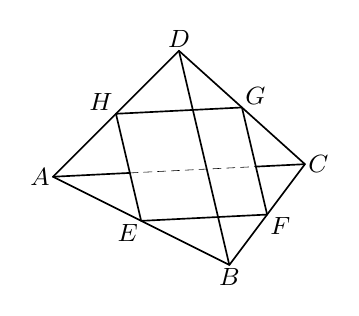
\begin{tikzpicture}[>=latex,scale=0.8,inner sep=1pt]
  \tkzDefPoints{0/0/A,2.8/-1.4/B,4/0.2/C,2/2.0/D}
  \tkzDefMidPoint(A,B)\tkzGetPoint{E}
  \tkzDefMidPoint(B,C)\tkzGetPoint{F}
  \tkzDefMidPoint(C,D)\tkzGetPoint{G}
  \tkzDefMidPoint(D,A)\tkzGetPoint{H}
  \tkzInterLL(A,C)(F,G)\tkzGetPoint{N}
  \tkzInterLL(A,C)(E,H)\tkzGetPoint{M}
  \tkzDrawPolygon[semithick](A,B,C,D)
  \tkzDrawPolygon[semithick](E,F,G,H)
  \tkzDrawSegments[semithick](B,D A,M N,C)
  \tkzDrawSegments[densely dashed](M,N)
  \tkzLabelPoints[below left](E)
  \tkzLabelPoints[below right](F)
  \tkzLabelPoints[left](A)
  \tkzLabelPoints[below](B)
  \tkzLabelPoints[above right](G)
  \tkzLabelPoints[right](C)
  \tkzLabelPoints[above](D)
  \tkzLabelPoints[above left](H)
\end{tikzpicture}
\end{document}